\documentclass[10pt]{article}
\setlength{\parskip}{0.25\baselineskip}
\usepackage[margin=1in]{geometry} 
\usepackage{amsmath,amsthm,amssymb, graphicx, multicol, array}
\usepackage[font=small,labelfont=bf]{caption}
\usepackage{float}

\newcommand{\supp}{{\text{supp}}} 
\newcommand{\bv}{{\text{BV}}}
\newcommand{\ac}{{\text{AC}}}

\newenvironment{problem}[2][]{\begin{trivlist}
\item[\hskip \labelsep {\bfseries #1}\hskip \labelsep {\bfseries #2.}]}{\end{trivlist}}

\begin{document}
 
\title{Homework \#3}
\author{Eric Tao\\
Math 123: Homework \#3}
\maketitle

\begin{problem}{Question 1}
Let $x,y \in \mathbb{R}^{d \times 1}$. Prove that $xy^T \in \mathbb{R}^{d \times d}$ has at most rank 1.

\end{problem}
\begin{proof}[Solution]

First, assume we're not in the degenerate case $x = 0$ or $y = 0$, as if either are true, then $xy^T = 0$, the 0 matrix.

Here, we recall that, by definition:

$$(xy^T)_{ij} = \sum_{k=1}^1 x_{ik}y_{kj} = x_i y_j$$ where I drop the second index because, of course, these are vectors. Fix some $i$. Then, looking at the $i$-th row, we notice that we may factor $x_i$ from every term. In particular, as a vector, the $i$-th row looks like:

$$ \begin{pmatrix} x_i y_1 & x_i y_2 & ... & x_i y_d \end{pmatrix} =  x_i \begin{pmatrix} y_1 & y_2 & ... & y_d \end{pmatrix} $$

where we notice that the $i$-th row is a multiple of $y$, as a row vector. Since the choice of $i$ was completely arbitrary, this process can be done for every row, and thus every row vector is a multiple of $y$. Thus, the row space has dimension 1, and since we're a square matrix, we have that the dimension of the row space is equal to that of the column space, and the rank is 1.

\end{proof}

\begin{problem}{Question 2}
Prove that the Euclidean dot product $\langle x, y \rangle = \sum_{i=1}^n x_i y_i, x, y \in \mathbb{R}^n$ is an inner product, where an inner product is a binary function from a (real-valued) vector space $V$ to a field $F$, $\langle \cdot, \cdot \rangle: V \times V \to F$ such that the following hold (in the context of a real vector space):

(a) For all $x,y \in V$, $\langle x,y \rangle =\langle y,x \rangle$

(b) For all $x,y \in V$, $\langle \alpha x,y \rangle =\alpha \langle x,y \rangle$

(c) For all $x,y, z \in V$, $\langle  x + y,z \rangle =\langle x,z \rangle + \langle y,z \rangle$

(d) For all $x\in V$, $\langle x,x \rangle \geq 0$ and $\langle x,x \rangle = 0 \iff x = 0$

\end{problem}

\begin{proof}[Solution]

(a) 

This should be clear by the commutativity of real numbers:

$$ \langle x, y \rangle = \sum_{i=1}^n x_i y_i = \sum_{i=1}^n y_i x_i = \langle y, x \rangle$$

(b)

This should be clear by how multiplication distributes over addition:

$$ \langle \alpha x, y \rangle = \sum_{i=1}^n (\alpha x_i) y_i = \alpha \sum_{i=1}^n y_i x_i = \alpha \langle y, x \rangle$$

(c) 

Same as (b), follows from distributive property of multiplication:

$$ \langle x+y, z \rangle = \sum_{i=1}^n (x_i + y_i) z_i = \sum_{i=1}^n x_i z_i + y_i z_i = \sum_{i=1}^n x_i z_i + \sum_{j=1}^n y_j z_j  = \langle x, z \rangle + \langle y, z \rangle$$

(d) 

First, we consider the expansion of $\langle x ,x \rangle$:

$$\langle x ,x \rangle = \sum_{i=1}^n x_i x_i = \sum_{i=1}^n x_i^2$$

Since we have that for all $x_i \in \mathbb{R}$, $x_i^2 \geq 0$, we have that $ \sum_{i=1}^n x_i^2$ is a sum of non-negative numbers, and thus must be at least 0. Thus, $\langle x ,x \rangle \geq 0$

It is obvious that if $x = 0$, then $\langle x, x \rangle = \sum_{i=1}^n 0 * 0  =0$. Now, suppose $\langle x, x \rangle = 0$. Then, we have that $ \sum_{i=1}^n x_i^2 = 0$. Since, again, these are non-negative numbers, this can only be 0 if $x_i = 0$ for all $i$. But, if $x_i  = 0$ for all $i$, $x$ is the $0$ vector.


\end{proof}

\begin{problem}{Question 3}

(a) Prove that $\langle x,y\rangle_M = x M y^T$ satisfies the properties of an inner product if $M$ is positive definite.

(b) Show that $\langle x,y\rangle_M$ need not be an inner product if $M$ is positive semi-definite.

\end{problem}

\begin{proof}[Solution]

(a)

Suppose $M$ is positive definite. We check each property in turn:

$$\langle x,y\rangle_M =  x M y^T = (x M y^T)^T = y M^T x^T = y M x^T = \langle y,x\rangle_M$$

where we use the fact that since $x M y^T$ is a scalar, and thus may be intepreted as a $1 \times 1$ matrix, it must be symmetric, and that $M$ being positive-definite means that $M$ is symmetric.

$$\langle \alpha x,y\rangle_M =  (\alpha x) M y^T = \alpha(x M y^T) = \alpha \langle x,y\rangle_M$$

where we use the fact that we can pull scalars out from matrix multiplication.

$$ \langle x+y, z \rangle_M  = (x+y) M z^T = xMz^T  + yMz^T = \langle \alpha x,z\rangle_M + \langle \alpha y,z\rangle_M $$

where we use the fact that matrix multiplication distributes over matrix addition.

and the last property comes by the definition of positive definite, as by definition, $x M x^T \geq 0$ for all $x$, and is 0 if and only if $x = 0$. So we notice that:

$$ \langle x, x \rangle_M = x M x^T \geq 0$$

and $$ \langle x,x \rangle = 0 \iff xM x^T = 0 \iff x = 0$$

So,  $\langle x,y\rangle_M$ defines an inner product.

(b)

We show a counter example. Consider the matrix:

$$A =   \begin{pmatrix} 1 & 0 \\ 0 & 0 \end{pmatrix}$$

It should be clear that this matrix is positive semi-definite because we may compute the characteristic polynomial and eigenvalues as $(1-\lambda) \lambda = 0 \implies \lambda = 0, 1 \geq 0$, and since $A$ is symmetric, with non-negative eigenvalues, it must be positive semi-definite.

However, this matrix does not define a inner product. Consider the vector $ v = \begin{pmatrix} 0 & 1 \end{pmatrix}$. We have that:

$$  v A v^T = \begin{pmatrix} 0 & 1 \end{pmatrix} \begin{pmatrix} 1 & 0 \\ 0 & 0 \end{pmatrix} \begin{pmatrix} 0 \\ 1\end{pmatrix} =   \begin{pmatrix} 0 & 1 \end{pmatrix}\begin{pmatrix} 0 \\ 0\end{pmatrix} = 0$$

Thus, because we found a non-0 $v$ such that $ v A v^T = 0$, we have that $v A v^T  = 0 \nRightarrow v = 0$, and thus we do not satisfy the biconditional.

\end{proof}

\begin{problem}{Question 4}

Let $x_1,...,x_n \in \mathbb{R}^d$. Fix some positive integer $K$. Let $C_1,...,C_K$ be a partition of the data with centroids $\mu_1,...,\mu_K$. Let

$$ F(C_1,...,C_k)  \sum_{k=1}^K \sum_{x_i \in C_K} \Vert \mu_k - x_i \Vert_2^2 $$

(a) Prove that, for a fixed $K$, $F$ achieves a minimum value.

(b) What is the minimum value if $K = n$?

\end{problem}

\begin{proof}[Solution]

(a)

Fix some $K \in \mathbb{N}$. Since $n$ is a fixed natural number, we have finitely many data points. In particular, if we have finitely many data points, then we can only have finitely many partitions of $n$ into $K$ subsets. Then, if we consider the values of $F_i$, where we index a partition $\Gamma_i$ by $i$, this is a set of non-negative real numbers, finite. By the least upper bound property of the real numbers, this must have an infimum since this is bounded below by $0$, and further, since this is a finite set, it must achieve the infimum, since finite sets do not have limit points. Thus, $F$ must achieve a minimum for fixed values of $K$.

(b)

If $K= n$, then we allow only the partition$C_1 = \{x_1\}, C_2 = \{ x_2 \} ... C_n = \{ x_n \}$ up to relabeling, since we have $n$ data points and $n$ boxes. Then, the centroid of each is exactly $\mu_j = x_j$, so then we have that for each $C_n$, that $$\sum_{x_i \in C_j  } \Vert \mu_j - x_i \Vert_2^2 = \Vert x_j - x_j \Vert_2^2 = 0$$ 

Thus, $F = \sum_{K=1}^n 0 = 0$, and the minimum and only value of $F$ if $K = n$ is $0$. And since the minimum value of a sum of non-negative real values is $0$, this must be the minimum value.


\end{proof}

\begin{problem}{Question 5}
 
Run the MATLAB script 'Kmeans\_Gaussians'.

(a) Run $K$-means with $K=2, 100$ replicates. Show the output visually.

(b) Plot the error of the $K$-means functional as a function of the number of iterations. Is there convergence?

(c) Do the clusters agree with your intuition?

\end{problem}

\begin{proof}[Solution]

Fixing a set of outputs from the Gaussians, we use the kmeans method built into matlab. Over 100 iterations, we find replicates that look like this:


\begin{figure}[H]
\centering
\begin{minipage}{.5\textwidth}
  \centering
  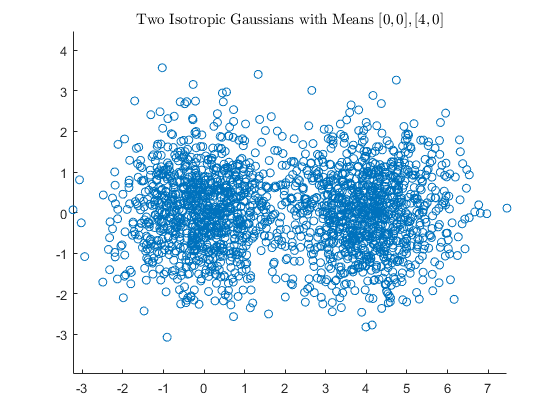
\includegraphics[width=\linewidth]{gaussian_points}
  \captionof{figure}{Gaussian points}
  \label{fig:test1}
\end{minipage}%
\begin{minipage}{.5\textwidth}
  \centering
  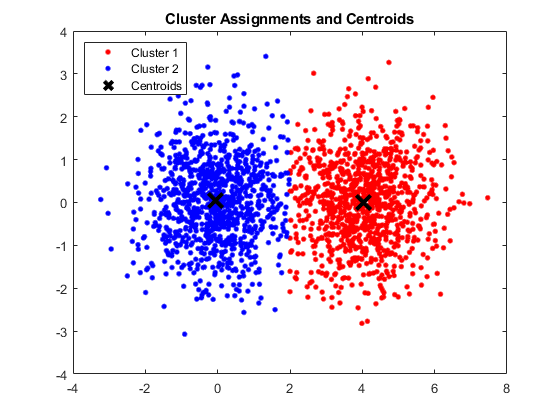
\includegraphics[width=\linewidth]{gaussian_cluster_assignments}
  \captionof{figure}{Gaussian points with Centroids and Cluster assignments}
  \label{fig:test2}
\end{minipage}
\end{figure}

Additionally, we had good agreement on the total error across replicates:

\begin{center}
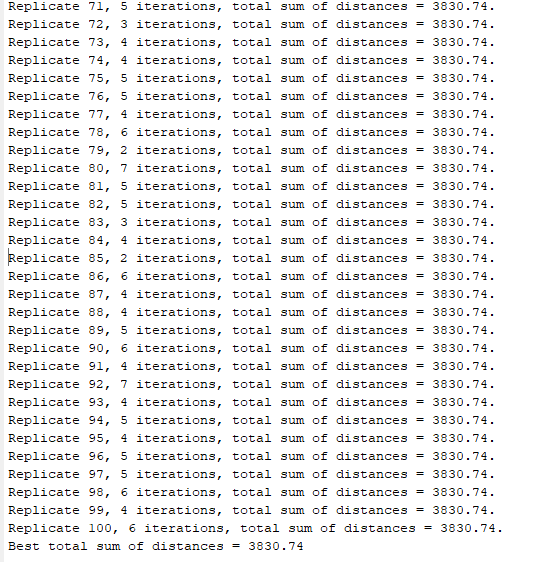
\includegraphics[,scale=0.5]{gaussian_iterations}
\captionof{figure}{}
\end{center}

Now, this time we specify a value for MaxIter, and record the best total sum of distances as a function of the max iterations, over a single replicate. We do this for 1-10, as we noticed that convergence happened in the 100 replicants within usually 6 iterations and graph total error against MaxIter:

\begin{center}
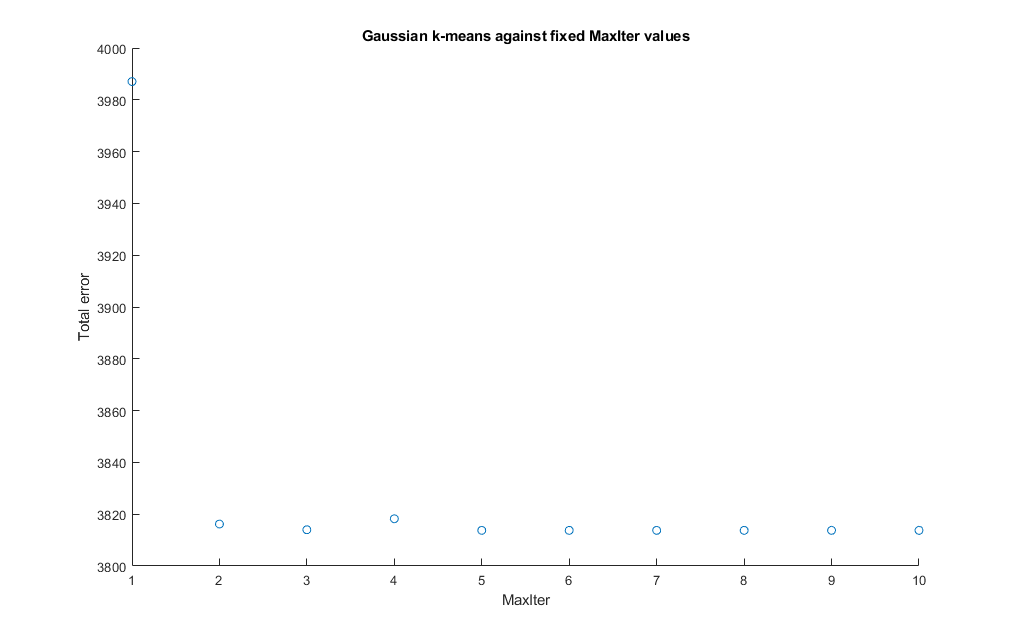
\includegraphics[,scale=0.5]{maxiter_against_total_error_gaussian}
\captionof{figure}{}
\end{center}

Visually at least, it seems like it converges reasonably after the first few iterations to an error of around 3820.

The clusters, as seen in figure 2, agree with our intuition. The code generated samples from a normal distribution centered on $(0,0)$ and then $(4,0)$. We then expect in two clusters, that our centroids would land on our means, which they do.

\end{proof}

\begin{problem}{Question 6}
 
Run the MATLAB script 'Kmeans\_Ellipses'.

(a) Run $K$-means with $K=2, 100$ replicates. Show the output visually.

(b) Plot the error of the $K$-means functional as a function of the number of iterations. Is there convergence?

(c) Do the clusters agree with your intuition?

\end{problem}

\begin{proof}[Solution]

Fixing a set of outputs from the ellipses, we use the kmeans method built into matlab. Over 100 iterations, we find replicates that look like this:


\begin{figure}[H]
\centering
\begin{minipage}{.5\textwidth}
  \centering
  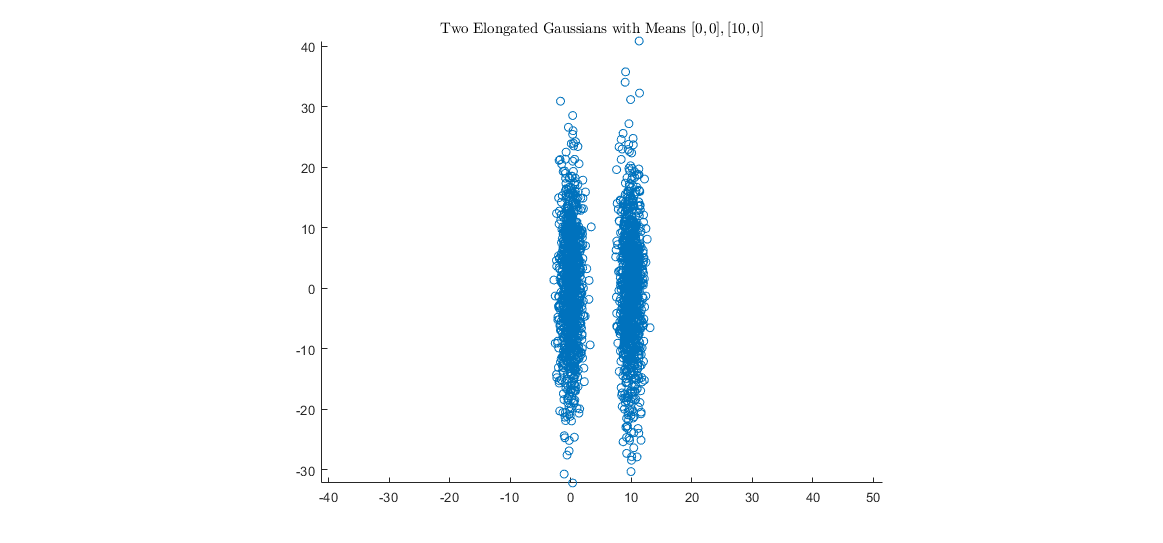
\includegraphics[width=\linewidth]{ellipse_points}
  \captionof{figure}{Ellipse points}
  \label{fig:test1}
\end{minipage}%
\begin{minipage}{.5\textwidth}
  \centering
  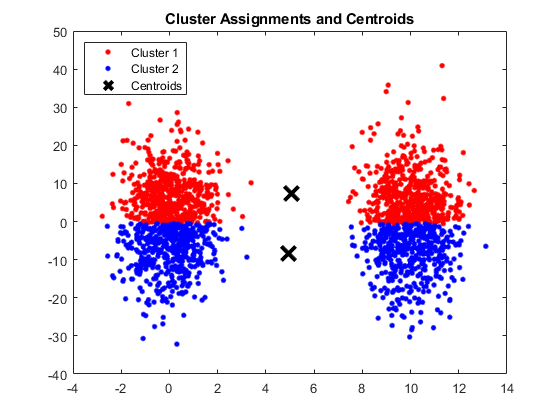
\includegraphics[width=\linewidth]{ellipse_cluster_assignments}
  \captionof{figure}{Ellipse points with Centroids and Cluster assignments}
  \label{fig:test2}
\end{minipage}
\end{figure}

Additionally, we had good agreement on the total error across replicates, though we notice some variance in the convergence as compared to the last problem:

\begin{center}
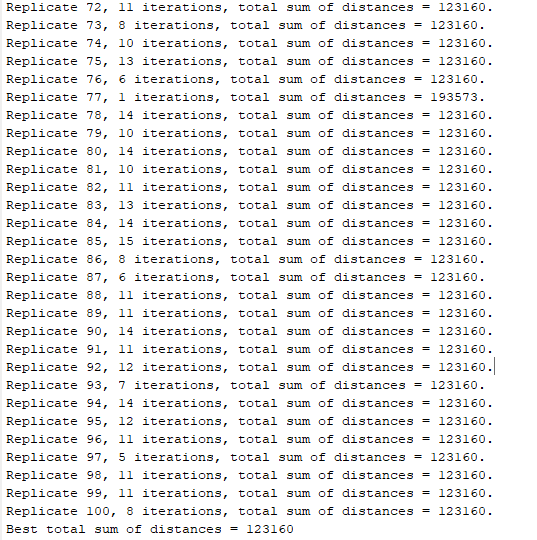
\includegraphics[,scale=0.5]{ellipse_iterations}
\captionof{figure}{}
\end{center}

Now, this time we specify a value for MaxIter, and record the best total sum of distances as a function of the max iterations, over a single replicate. We do this for 1-20, because many of the 100 replicants required more than 12 iterations to converge and graph total error against MaxIter:

\begin{center}
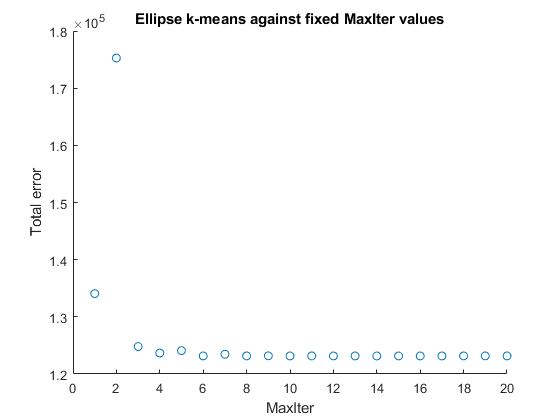
\includegraphics[,scale=0.5]{maxiter_against_total_error_ellipse}
\captionof{figure}{}
\end{center}

Visually at least, it seems like it converges reasonably after the first few iterations to an error of around 123160, though we notice a bit more variance at low iteration counts than in the Gaussian case.

The clusters, as seen in figure 2, do not really agree with our intuition, since we see visually that the scatterplot resembles two ellipses, but if we minimize the error, the best partition is actually by partitioning the data points along the elongated major axis. In a sense, due to how elongated our ellipses are, these choices of centroids, and not the centers of the ellipses, capture more of the variance.


\end{proof}

\end{document}